\section{Interfaz}
\begin{itemize}
	\item Sistema visual
	      \begin{figure}[htb]
		      \centering
		      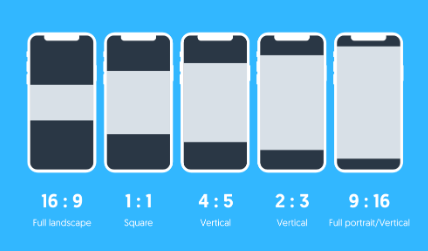
\includegraphics[width=0.95\textwidth]{Figures/0. General/sistema_visual.png}
		      \caption{Modelo a usar 9:16 vertical $1080 \times 1920$}
		      \label{fig:vista}
	      \end{figure}
	\item HUD - controles: Panel táctil (Android)
	      \begin{figure}[h!]
		      \centering
		      \begin{subfigure}[b]{0.35\linewidth}
			      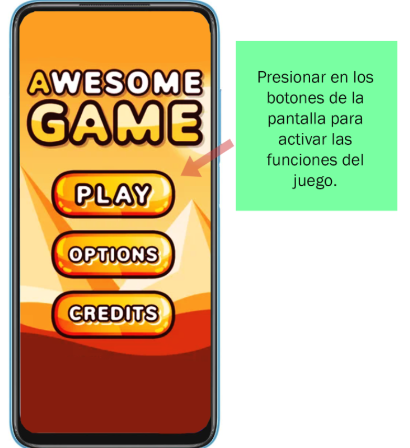
\includegraphics[width=\linewidth]{Figures/0. General/phone.png}
			      \caption{Referencia de tactil}
			      \label{fig:westminster_lateral}
		      \end{subfigure}
		      \begin{subfigure}[b]{0.45\linewidth}
			      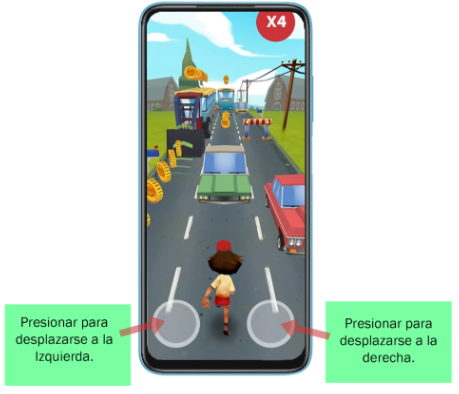
\includegraphics[width=\linewidth]{Figures/0. General/phone_2.png}
			      \caption{Referencia de interfaz}
			      \label{fig:westminster_aerea}
		      \end{subfigure}
		      \caption{Mecanica de movimientos}
		      \label{fig:westminster}
	      \end{figure}
	      \begin{itemize}
		      \item Menús: Sistema de inicio de juego (Iniciar/ Opiones/ Salir)
		      \item Sistema de Rendering: Pausa (Opiones/ Volumen/ Menú)
		      \item Cámara: Cámara tercera persona
		      \item Modelos de luz: Iluminación variada entre poca luz a oscuridad.
	      \end{itemize}
	\item Sistema de control - ¿Cómo el jugador controla el juego? ¿Cuáles son los controles especificos?
	\item Audio: Música ambientar de bosque nocturno
	\item Música: Música de suspenso
	\item Efectos de sonido: Efectos de sonido de pisadas en un suelo de madera, pavimento y tierra.
\end{itemize}

\section{Inteligencia Artificial}
\begin{itemize}
	\item IA de oponente - el oponente activo que está en contra del jugador y sus estrategias
	      logramos que el enemigo persiga al protagonista, utilizando el NavMesh que es una IA de
	      movimientos inteligentes por un área determinada, siendo que esta esta presente en Unity.
\end{itemize}

\section{Elementos técnicos}
\subsection{Hardware objetivo}
Run or Wake tiene como objetivo a un público que disponga de un celular Android. Para una mejor
experiencia de juego recomendamos las siguientes características:
\begin{itemize}
	\item Procesador: Se requiere un procesador de gama baja exynos 7884, octa core a 1.6GHz
	\item Memoria RAM: Se recomienda una memoria de 2GB de RAM, ya que es importante para almacenar
	      los datos y procesos que están en funcionamiento.
	\item Almacenamiento: El almacenamiento se recomienda 25GB, ya que se va a almacenar los datos
	      del juego y el proceso en forma local.
	\item Conectividad: Asegurarse de tener una conexión necesaria de internet para ingresar al juego.
\end{itemize}

\subsection{ Procedimientos de desarrollo y estándares}
Para el desarrollo del videojuego contamos con 8 miembros quienes al usar Jira y GitHub tendremos objetivos
definidos por fechas.

\subsection{Game engine}
El motor de desarrollo como base es Unity ya que a diferencia de Unreal Engine no tiene tanto
peso al momento de desarrollar, siendo que el jeugo no necesita de una gráfica ultra realistas,
y más que nuestro juego es estilo LowPoly.

\subsection{Network}
Si requiere conexión a internet para la descarga del mismo como para ingresar a un registro mediante
un login, pero el juego es sin conexión.
\subsection{Lenguaje de scripting}
El Lenguaje de programación que se usará para desarrollar el proyecto es C\#.

\section{Arte del juego}

Esto será tratado de forma breve, siendo más detallado en la biblia de arte.

\begin{itemize}
	\item Concept art: Estilo caricaturesco
	\item Guías de estilo: Utilizamos el estilo LowPoly que se aplica al escenario y objetos del juego
	\item Diseño de personajes: Nos enfocamos en la simplicidad pero con caracter de colores vivos.
	\item Escenarios: Contamos con paisajes naturales y de urbe, es decir una ciudad y un bosque, todo esto
	      manteniendo la estetica LowPoly.
\end{itemize}

\section{Software secundario}
\begin{itemize}
	\item Editor: Visual Studio (Microsoft), Jira Software, Unity, GitHub, Adobe Photoshop, Blender, Zbrush,
	      Neovim.
	\item Instalador: Unity.exe - Unity.deb
	\item Update Software: Versión 2022.3.3
\end{itemize}

\section{Manejo}
\subsection{Calendario Detallado}
\begin{enumerate}[label=Semana \arabic*:, align=left, leftmargin=*]
\item (20 de junio - 26 de junio):
\begin{itemize}[label=--]
	\item Definir el concepto y la mecánica básica del juego.
	\item Crear un documento de diseño inicial.
	\item Realizar bocetos y prototipos de los niveles del juego.
	\item Investigar y seleccionar las herramientas de desarrollo adecuadas.
\end{itemize}

\item (27 de junio - 3 de julio):
\begin{itemize}[label=--]
	\item Comenzar la creación de los modelos 3D para los personajes y objetos del juego.
	\item Diseñar los primeros niveles y establecer su estructura básica.
	\item Investigar y seleccionar los recursos visuales y de audio necesarios para el juego.
\end{itemize}

\item (4 de julio - 10 de julio):
\begin{itemize}[label=--]
	\item Continuar con la creación de los modelos 3D y texturas.
	\item Implementar la lógica básica del juego.
	\item Crear los primeros prototipos de los controles y la interfaz de usuario.
\end{itemize}

\item (11 de julio - 17 de julio):
\begin{itemize}[label=--]
	\item Refinar los modelos 3D y texturas existentes.
	\item Desarrollar los niveles con mayor detalle y agregar elementos interactivos.
	\item Implementar las mecánicas de juego adicionales, como la detección de colisiones y la física básica.
\end{itemize}

\item (18 de julio - 24 de julio):
\begin{itemize}[label=--]
	\item Añadir efectos visuales y de sonido al juego.
	\item Realizar pruebas de juego y corregir errores.
	\item Optimizar el rendimiento del juego.
\end{itemize}

\item (25 de julio - 31 de julio):
\begin{itemize}[label=--]
	\item Crear una pantalla de inicio y una pantalla de "game over".
	\item Implementar el sistema de puntuación y progreso del jugador.
	\item Ajustar el equilibrio del juego y mejorar la jugabilidad según las pruebas realizadas.
\end{itemize}

\item (1 de agosto - 7 de agosto):
\begin{itemize}[label=--]
	\item Realizar pruebas finales y solucionar cualquier problema pendiente.
	\item Pulir los detalles visuales y de sonido.
	\item Preparar el juego para su lanzamiento final.
\end{itemize}

\item (8 de agosto):
\begin{itemize}[label=--]
	\item Lanzamiento del juego.
	\item Realizar una campaña de promoción para dar a conocer el juego.
\end{itemize}
\end {enumerate}

\subsection{Presupuesto}
\begin{enumerate}
	\item Desarrollador principal (x1): \$40 por hora x 400 horas estimadas de trabajo = \$16,000
	\item Diseñador de juegos (x1): \$35 por hora x 300 horas estimadas de trabajo = \$10,500
	\item Artista 3D (x2): \$30 por hora x 250 horas estimadas de trabajo (por artista) = \$15,000
	\item Programador (x2): \$35 por hora x 250 horas estimadas de trabajo (por programador) = \$17,500
	\item Diseñador de sonido (x1): \$30 por hora x 200 horas estimadas de trabajo = \$6,000
	\item Testers/QA (x1): \$25 por hora x 200 horas estimadas de trabajo = \$5,000
\end{enumerate}

\textbf{2. Software y licencias:}
\begin{itemize}
	\item Unity (versión gratuita): sin costo.
	\item Software libre y herramientas gratuitas: sin costo.
	\item Plugins y assets gratuitos de la Asset Store de Unity: sin costo o costo mínimo, dependiendo de los recursos utilizados.
\end{itemize}

\textbf{3. Hardware y equipo de trabajo:}
\begin{itemize}
	\item Computadoras: ya en posesión del equipo.
	\item Licencias de desarrollo y consolas de juego (si aplica): verificar los requisitos específicos y los costos asociados.
\end{itemize}

\textbf{4. Recursos externos:}
\begin{itemize}
	\item Música y efectos de sonido: presupuesto variable según los acuerdos y el alcance del proyecto. Por ejemplo, \$2,000.
\end{itemize}

\textbf{5. Gastos generales:}
\begin{itemize}
	\item Espacio de trabajo, electricidad, internet, etc. Por ejemplo, \$1,000.
\end{itemize}

\textbf{6. Contingencia:}
\begin{itemize}
	\item 15\% del costo total estimado del proyecto (suma de los salarios del equipo + recursos externos + gastos generales). Por ejemplo, si el costo total estimado es de \$60,000, la contingencia sería de \$9,000.
\end{itemize}

El costo total estimado del proyecto sería la suma de los salarios del equipo, los recursos externos, los gastos generales y la contingencia:

\textbf{Costo total estimado del proyecto:}

\[\$16,000+\$10,500+\$15,000+\$17,500+\$6,000+\$5,000+\$2,000+\$1,000+\$9,000=\$82,000\]

\subsection{Análisis de riesgo}

\begin{enumerate}
	\item Problemas Técnicos
	      \begin{itemize}
		      \item El juego tiene muchos bugs y errores.
	      \end{itemize}

	\item Problemas de Diseño
	      \begin{itemize}
		      \item La calidad del diseño no es la mejor y no es agradable a la vista, lo que genera molestias.
	      \end{itemize}

	\item Problemas de Producción
	      \begin{itemize}
		      \item Conflictos con el uso de la herramienta git y github.
	      \end{itemize}

	\item Problemas de Marketing
	      \begin{itemize}
		      \item No hay presupuesto para hacer publicidad en plataformas oficiales.
	      \end{itemize}

	\item Problemas de Tiempo de desarrollo
	      \begin{itemize}
		      \item El proyecto no se logra terminar en el tiempo establecido.
	      \end{itemize}

	\item Clasificación de los Riesgos
	      \begin{itemize}
		      \item Riesgo Bajo: Problemas de tiempo de desarrollo, problemas de marketing.
		      \item Riesgo Medio: Problemas de Producción, Problemas de diseño.
		      \item Riesgo Alto: Problemas Técnicos por su impacto y alta probabilidad, debido a la falta de experiencia en el desarrollo.
	      \end{itemize}

	\item Evaluación de Riesgos
	      \begin{itemize}
		      \item Riesgo Bajo: El riesgo bajo tiene una tasa de probabilidad del 10% ya que contamos con un plan de desarrollo con una ventaja en el tiempo.
		      \item Riesgo Medio: El riesgo medio tiene una tasa de probabilidad del 30%. Nuestro equipo tiene poca experiencia utilizando la herramienta git.
		      \item Riesgo Alto: El riesgo alto tiene una probabilidad del 45% ya que no tenemos experiencia en el desarrollo.
	      \end{itemize}
\end{enumerate}

\subsection{Gestión de Riesgos}
\begin{itemize}
	\item Riesgo Bajo:
	      Utilizamos la aplicación de Jira para poder organizarnos y tener un control del tiempo de desarrollo. Utilizamos pequeños objetivos y administramos roles y deberes o encargos.

	\item Riesgo Medio:
	      Haremos uso de assets desarrollados por otros que nos dan de manera gratuita, con la condición de mencionarlos en los créditos del juego.
	\item Riesgo Alto Haremos uso de la Documentación de Unity y los foros de desarrolladores como

	      StackOverflow, comunidad de desarrollo y en caso de no poder solucionar, pediremos ayuda a

	      nuestro instructor de curso.
\end{itemize}

\begin{figure}[!ht]
	\centering
	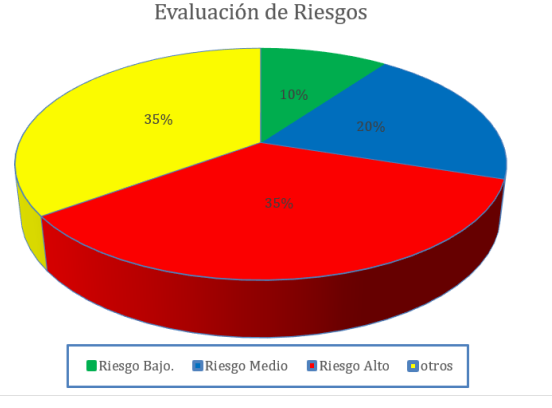
\includegraphics[width=0.5\textwidth]{Figures/0. General/riesgos.png}
	\caption{Porcentajes de riesgos}
	\label{fig:riesgos}
\end{figure}

\subsection{Planes de localización}
\subsubsection{Indentificación de los idiomas y culturas}
El juego está destinado a la comunidad Latinoamericana Hispanohablantes, por lo cual el idioma es el español.
\subsubsection{Selección de equipos de localización}
Somos 8 Desarrolladores nacidos en Latinoamérica Hispanohablantes de lengua materna.
\subsubsection{Adaptación del contenido del juego}
Debemos de adaptar todo el contenido del juego, idiomas y culturas. Esto incluye traducir el texto y los diálogos, adaptar gráficos, elementos visuales y asegurarnos de que el juego cumpla con las normas regulaciones de cada país objetivo.
\subsubsection{Pruebas y revisión}
Una vez finalizada la adaptación del juego, es necesario realizar pruebas exhaustivas para asegurarse de que todo funciona correctamente de esta manera nuestro juego es atractivo para el Público objetivo, también debemos revisar el juego para detectar y corregir cualquier error o problema que pueda haber.
\subsubsection{Lanzamiento del juego}
Para finalizar, una vez que el juego ha sido adaptado y probado, está listo para ser lanzado al mercado

\subsection{Plan de test}

\subsection{Objetivo}
Nuestro objetivo principal es el correcto funcionamiento de nuestro juego con el fin de entretener a nuestro público general y recibir opiniones positivas en la plataforma donde se va a descargar o subir (Play Store, etc.).

\subsection{Estrategia de Prueba}
Se llevarán a cabo pruebas de caja blanca y pruebas de caja negra. También se realizarán pruebas de rendimiento y carga para evaluar el rendimiento del juego.

\subsection{Requisitos de Prueba}
\begin{itemize}
	\item El juego será probado en una variedad de dispositivos móviles de diferentes gamas, capacidades y estructuras.
	\item El juego debe ejecutarse sin problemas en dispositivos Android.
	\item Se deben realizar pruebas de rendimiento.
\end{itemize}

\subsection{Casos de Prueba}
\begin{enumerate}
	\item \textbf{Prueba 1: Inicio y cierre del juego en dispositivos Android}

	      \textbf{Escenario:} El jugador inicia y cierra en un dispositivo móvil.

	      \textbf{Pasos:}
	      \begin{enumerate}
		      \item Inicie el juego en un dispositivo móvil.
		      \item Cierre el juego.
	      \end{enumerate}

	      \textbf{Resultado esperado:} El juego inicia y cierra sin problemas.

	\item \textbf{Prueba 2: Uso del menú principal en dispositivos de escritorio}

	      \textbf{Escenario:} El jugador navega por el menú principal del juego en un dispositivo móvil.

	      \textbf{Pasos:}
	      \begin{enumerate}
		      \item Inicie el juego en un dispositivo de escritorio.
		      \item Navegue por el menú principal del juego.
	      \end{enumerate}

	      \textbf{Resultado esperado:} El menú principal se muestra correctamente y se puede navegar sin problemas.

	\item \textbf{Prueba 3: Uso del menú de opciones en dispositivos de escritorio}

	      \textbf{Escenario:} El jugador navega por el menú de opciones del juego en un dispositivo móvil.

	      \textbf{Pasos:}
	      \begin{enumerate}
		      \item Inicie el juego en un dispositivo móvil.
		      \item Navegue por el menú principal del juego.
		      \item Navegue por el menú de opciones del juego.
	      \end{enumerate}

	      \textbf{Resultado esperado:} El menú de opciones se muestra correctamente y se puede navegar sin problemas.

	\item \textbf{Prueba 4: Uso del menú de perfil en dispositivos de escritorio}

	      \textbf{Escenario:} El jugador navega por el menú de perfil del juego en un dispositivo móvil.

	      \textbf{Pasos:}
	      \begin{enumerate}
		      \item Inicie el juego en un dispositivo móvil.
		      \item Navegue por el menú principal del juego.
		      \item Navegue por el menú de perfil del juego.
	      \end{enumerate}

	      \textbf{Resultado esperado:} El menú de perfil se muestra correctamente y se puede navegar sin problemas.

	\item \textbf{Prueba 5: Uso del juego en dispositivos de escritorio}

	      \textbf{Escenario:} El jugador navega por el menú principal, accede al juego y procede a jugar en un dispositivo móvil.

	      \textbf{Pasos:}
	      \begin{enumerate}
		      \item Inicie el juego en un dispositivo móvil.
		      \item Navegue por el menú principal del juego.
		      \item Presione "Jugar".
	      \end{enumerate}

	      \textbf{Resultado esperado:} El jugador accede sin problemas al juego y no encuentra fallas en el juego.

\end{enumerate}

\section{Apéndices}
\textbf{Arte}

\begin{enumerate}
	\item Modelado y lista de texturas
	\item Lista de animaciones
	\item Lista de efectos
	\item Lista de arte de la interfaz
	\item Lista de cortes de escenas
\end{enumerate}

\textbf{Sonido}

\begin{enumerate}
	\item Sonidos ambientales
	\item Sonidos de interfaz
	\item Sonidos de eventos
\end{enumerate}

\textbf{Música}

\begin{enumerate}
	\item Ambiente
	\item Acción
	\item Victoria
	\item Muerte o pérdida
\end{enumerate}
\newpage
Todos los recursos mencionados anteriormente los tenemos en OneDrive
\begin{figure}
	\centering
	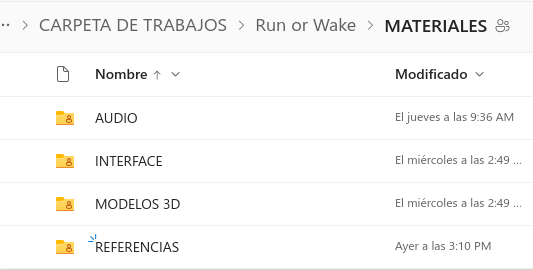
\includegraphics[width=1\textwidth]{Figures/0. General/apendice.png}
	\caption{Recursos de Apendice}
	\label{fig:apendice}
\end{figure}
